\chapter{Implementation\label{chap:implementation}}
This chapter will discuss the technical specifications of the project and discuss the decisions that affected the process. I will also overview my workflow and iterative approach to the project. Last, but not least, I will include and credit a list of third party libraries that this framework makes use of.

\section{Development process}

In this section I will outline how the work on my dissertation was conducted along with pointing out the pitfalls and making sure that project remains fully functional.

\subsection{Project plan}

\begin{figure}[h]
    \centering
    \makebox[\textwidth][c]{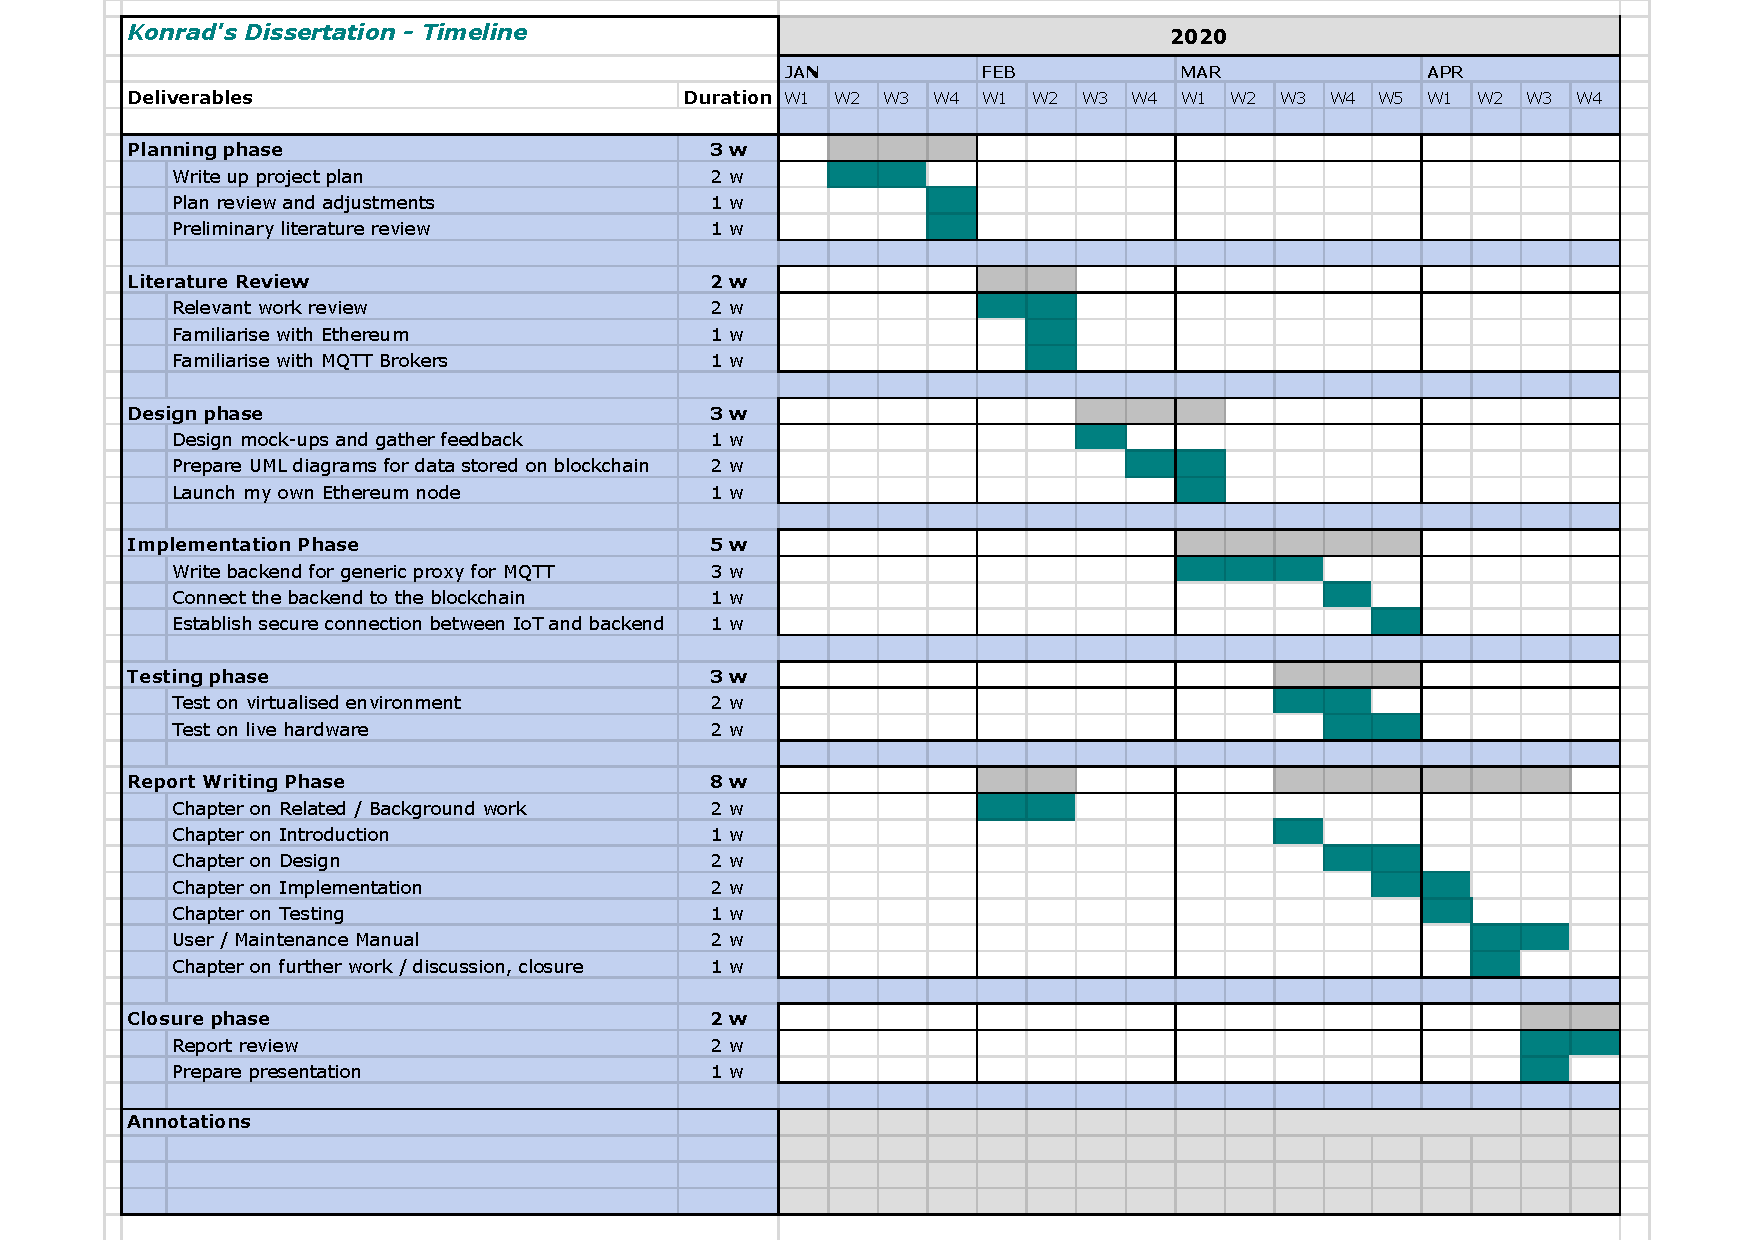
\includegraphics[width=1.1\textwidth]{timeline}}
    \caption{Project timeline}
    \label{fig:timeline}
\end{figure}

Figure \ref{fig:timeline} demonstrates the timeline of the project and all included phases. Each of those tasks was also divided onto smaller subsections (not shown on the diagram), which were worked on using agile approach, as described in the next section.

\subsection{Iterative Approach}

When designing my project plan, I distributed the workload onto small chunks and features which would have been implemented in an iterative way. I was following agile methodologies, dedicating each week on a different feature, where I would go through the entire development cycle for each unit. For example, generating the reports (section 4.4.2) was first introduced during a meeting with my supervisor, where I would establish the requirements and success criteria for this particular story. Then I would spend a day or two designing the flow and functionality, followed by an extra two days implementing designed features. At the very end, I would conduct testing and regression testing to make sure that the rest of the project still remains operational. This would have been concluded with a meeting with my supervisor to reflect on the sprint and determine whether success criteria were met.

\subsection{Regression testing}

Since I was following agile workflow when working on the project, it was important to ensure that none of the `stories' (or, tasks) affected each other when completed. I could have found myself in a situation where working on the reporting of the events to the blockchain might have broken another, unrelated feature, e.g. verifying the authenticity of connecting clients. That is the reason behind keeping regression testing as a vital phase of development. I was able to achieve it through continuous, automated testing - which includes unit, integration, regression and manual testing.

\section{Technologies}

In this subsection I will describe the technologies used in this project, that is, languages, frameworks, third party libraries and different approaches when it comes to writing the code.

\subsection{Languages used}

Following programming languages have been used when working on this project:
\begin{itemize}
 \item \textbf{Golang} - main driver behind the proxy, MQTT client and for communicating with the blockchain. It has also be used to write a simple backend for the web application.
 \item \textbf{Solidity} - language used to develop smart contracts on Ethereum.
 \item \textbf{HTML5 + CSS3 + JavaScript} - frontend stack used to create a website to display contents of blockchain.
 \item \textbf{Bash} - to design and execute tests capturing the latency of requests
\end{itemize}

\subsubsection{Golang}
Golang 
\subsubsection{Solidity}
\subsubsection{HTLM5 + CSS3 + JavaScript}
\subsubsection{Bash}

\subsubsection{Considered alternatives}

\subsection{Third party libraries \& resources}

\subsection{Working with Blockchain}

\subsection{Development tools}
\subsubsection{Version Control}
\subsubsection{Text Editor}

\subsection{Configuration}

\subsection{Logging}

